%% JVCI / Elsevier CAS single-column working manuscript.
%% Compile: pdflatex -> bibtex -> pdflatex -> pdflatex.
%% Replace every red TODO before submission and remove template-only comments.

\documentclass[a4paper,fleqn]{cas-sc}

\usepackage[numbers]{natbib}
\usepackage{amsmath}
\usepackage{amssymb}
\usepackage{booktabs}
\usepackage{graphicx}
\graphicspath{{figures/}}
\usepackage{xcolor}
\usepackage{url}

\newcommand{\todo}[1]{\textcolor{red}{[TODO: #1]}}
\newcommand{\evidence}[1]{\textcolor{blue}{[EVIDENCE: #1]}}

\begin{document}
\let\WriteBookmarks\relax
\def\floatpagepagefraction{1}
\def\textpagefraction{.001}

\shorttitle{Structured AIGC Provenance Verification}
\shortauthors{Dong and Luo}

\title[mode=title]{Structured DWT--DCT Payloads for Database-Backed AIGC Image
Provenance Verification and Trust Scoring}

\author[1]{Lianli Dong}[orcid=0009-0005-3415-3894]
\cormark[1]
\ead{3120233582@qq.com}

\author[1]{Zican Luo}
\ead{772358933@qq.com}
% TODO: add ORCID after confirmation.

\affiliation[1]{organization={School of Economics and Management, Hunan University of Technology},
  city={Zhuzhou},
  postcode={412007},
  state={Hunan},
  country={China}}

\cortext[1]{Corresponding author.}

\begin{abstract}
Artificial intelligence-generated content (AIGC) images can be edited and
redistributed after generation, yet an AI detector or a watermark bit string
does not establish that an image belongs to a registered generation event.
Watermarking, metadata, and perceptual hashing provide complementary evidence,
but they are often verified separately, leaving payload integrity, registry
identity, and image-content consistency unresolved within one decision. We
present a platform-controlled provenance framework that encodes projected
platform, generation, model-version, timestamp, and content fields, together
with a cyclic redundancy check (CRC-16), into a 128-bit payload. The record is
protected by a Reed--Solomon code, RS(32,16), and fourfold repetition, and 1024
coded bits are embedded using discrete wavelet and discrete cosine transforms
(DWT--DCT) on the luminance channel. Verification searches spatial alignments,
decodes the payload, matches its generation identifier against a trusted
registry, binds image content through oriented FAST and rotated BRIEF (ORB) or a
texture-aware fallback, and assigns graded trust. Acceptance requires payload
integrity, registered-generation matching, content agreement, and non-low
trust. On 200 registered and 100 clean negative images, mean PSNR was 39.65 dB
and SSIM was 0.998980; acceptance was 92.0\% for crop0.9 and 81.5\% for
crop+resize+JPEG70. Joint verification rejected all 20 tested forged and 50
transplanted payloads; the held-out area under the receiver operating
characteristic curve (AUC) was 0.999833. Strong screen-capture and print--scan
simulations remained unresolved at 0/200. These results support
platform-scoped provenance rather than universal cross-platform attribution.
\end{abstract}

% For preview only. The journal requires a separate editable Highlights file.
\begin{highlights}
\item A 128-bit structured payload links images to registered generation events.
\item DWT--DCT embedding achieved 39.65 dB PSNR and 0.99898 SSIM.
\item Joint verification rejected all 20 forged and 50 transplanted payloads.
\item Crop and compound JPEG cases reached 92.0\% and 81.5\% acceptance.
\item Screen-capture and print--scan simulators failed on all 200 test images.
\end{highlights}

\begin{keywords}
AIGC provenance \sep image watermarking \sep DWT--DCT \sep
perceptual hashing \sep trust scoring
\end{keywords}

\maketitle

\section{Introduction}\label{sec:intro}
Artificial intelligence-generated content (AIGC) has made the creation and
editing of realistic images routine, while separating an image from the
context in which it was produced. Content labels and provenance records are
therefore increasingly important to platform governance and consumer trust.
Labeling measures and technical standards define how generated content should
be disclosed \cite{ai_content_labeling_measures_2025,gb45438_2025}, and
provenance initiatives such as the Coalition for Content Provenance and
Authenticity (C2PA) provide structured manifests for source and editing
assertions \cite{noauthor_content_nodate,collomosse_authenticity_2024}.
Labeling alone, however, indicates that content is synthetic; it does not
necessarily identify the platform, model, or generation event that produced a
particular image.

This distinction turns provenance verification into a question of evidence
consistency rather than a binary AI-image classification. A detector may
estimate whether content is synthetic, and a watermark detector may indicate
that a mark is present, but neither result alone establishes that the image
belongs to a registered generation event. A metadata manifest can provide rich
context, yet its assertions may become separated from, or inconsistent with,
the pixels \cite{nemecek_authenticated_2026}. Conversely, a watermark can
survive common transformations and act as a compact identifier, but a
syntactically valid payload may be unregistered or may have been copied from a
different image \cite{saberi_drew_2024,jiang_watermark-based_2026}. Reliable
verification must therefore answer three separate questions: whether the
payload is intact, whether it identifies a trusted record, and whether the
query content agrees with that record.

Existing approaches provide strong but partial tools for these questions.
Transform-domain watermarking embeds information in perceptually significant
or multiresolution coefficients and supports blind extraction
\cite{cox_secure_1997,benoraira_blind_2015,najafi_robust_2017}. Learned and
generative watermarking improves payload recovery by training post-hoc encoders
or integrating fingerprints into the generation process
\cite{ferrari_hidden_2018,fernandez_stable_2023,xu_invismark_2025,gowal_synthid-image_2025}.
Provenance registries, error-controlled retrieval, perceptual hashes, and
user-level attribution move beyond mark presence by matching content or
identifiers against databases
\cite{saberi_drew_2024,jiang_watermark-based_2026,sharma_distance_2024,mohit_provenance_2026}.
These lines are usually optimized separately: watermark studies emphasize
imperceptibility and bit recovery, whereas registry studies emphasize content
retrieval or record management. This leaves an end-to-end gap between a
recovered structured record and a trustworthy platform-level verification
decision.

We address this gap with a platform-controlled provenance framework that
combines a compact structured payload, robust blind embedding, database
matching, content binding, and graded trust. Each generation event is
represented by a 128-bit record containing projected platform, generation,
model-version, timestamp, and content fields, together with CRC-16 protection.
The record is encoded with RS(32,16) and fourfold repetition and embedded into
the luminance channel using DWT--DCT coefficient differencing. At verification
time, the candidate search recovers the payload, matches its generation
identifier against the registry, compares the query content with the registered
source, and maps the combined evidence to a trust level. Acceptance requires
integrity, a registered generation match, successful content binding, and
non-low trust; the score remains available for diagnosis when attribution is
rejected.

This paper makes three bounded contributions.

\begin{enumerate}
  \item \textbf{Structured provenance payload.} We define a fixed-length
        multi-field record and a reproducible blind carrier that connects the
        payload to a registry while remaining suitable for post-hoc embedding.
  \item \textbf{Joint verification and calibrated trust.} We separate payload
        integrity, generation matching, content binding, and trust scoring, and
        evaluate the resulting verifier with forged and transplanted payloads
        in addition to registered positives.
  \item \textbf{Bounded robustness evidence.} We provide a controlled
        evaluation protocol covering image quality, error-corrected recovery,
        single and compound propagation, carrier and coding ablations,
        image-disjoint calibration, external baselines, and explicit physical
        failure cases.
\end{enumerate}

The approach targets provenance verification within participating platforms.
It is not a universal AI-image detector or an attribution mechanism across
unregistered platforms, and its ability to handle real screen capture and
print--scan propagation remains an open problem addressed only through bounded
stress simulations in this study.

\section{Related Work}\label{sec:related}

Research on AIGC traceability spans watermark design, generator integration,
metadata provenance, and robustness evaluation. Recent surveys describe rapid
progress in both the scope of these mechanisms and their unresolved security
and deployment questions \cite{cao_secure_2026,zhao_sok_2025,liu_review_2024,sun_generated_image_watermark_review_2026}.
The following subsections focus on the lines that determine the design of the
present verifier.

\subsection{Transform-Domain Image Watermarking}
Classical image watermarking treats the carrier image as a communication
channel and modifies selected spatial or transform-domain samples.
Spread-spectrum embedding distributes a pseudorandom watermark over perceptually
significant spectral components, trading capacity against imperceptibility and
robustness \cite{cox_secure_1997}. Multiresolution and block-frequency
representations provide complementary tools: DWT separates coarse structure
from detail, while the DCT concentrates local energy within blocks. Differential
DWT--DCT embedding compares transformed sub-vectors so that the sign of their
difference carries a bit without access to the host image
\cite{benoraira_blind_2015}. DWT-domain schemes have similarly demonstrated
blind extraction and resilience to selected signal-processing attacks
\cite{najafi_robust_2017}.

Adaptive and frequency-aware designs extend these principles to
authentication-oriented tasks. Hsu et al. embed auxiliary deepfake-detection
evidence with adaptive blind watermarking and recover it without side
information \cite{hsu_ai-assisted_2024}. Such methods show that transform-domain
carriers can balance image quality and post-processing robustness, but their
primary output is often a copyright mark, a detector signal, or a fixed
watermark message. They do not by themselves define how a multi-field decoded
record is matched to a trusted registry or how a valid mark is prevented from
being reassociated with different image content. The present method retains
the re-implementable advantage of blind coefficient-difference extraction, but
places it inside a structured provenance and joint-verification pipeline.

\subsection{Generative and Post-Hoc AIGC Watermarking}
Learned watermarking methods replace hand-designed coefficient rules with
encoder--decoder networks trained against differentiable distortions. HiDDeN
jointly learns data hiding and recovery \cite{ferrari_hidden_2018}, while
StegaStamp targets robust messages in printed and digitally displayed
photographs \cite{tancik_stegastamp_2020}. TrustMark uses a GAN-based encoder
and spatio-spectral losses for arbitrary-resolution images
\cite{bui_trustmark_2023}, and InvisMark emphasizes high-resolution AIGC
provenance with imperceptible embedding \cite{xu_invismark_2025}. These
post-hoc systems can operate after generation, which makes them applicable
across generators, but their learned extractors primarily optimize message
recovery or detection and do not establish registry or content consistency.

Model-integrated watermarking instead modifies the generation process. Stable
Signature fine-tunes the latent decoder so that generated images carry a
signature recoverable by a pretrained extractor
\cite{fernandez_stable_2023}. Tree-Rings embeds a fingerprint in the initial
noise and follows it through sampling \cite{wen_tree-rings_2023}, whereas
Gaussian Shading and Gaussian Shading++ construct distribution-preserving
watermarks while considering deployment and key-management constraints
\cite{yang_gaussian_2024,yang_gaussian_2025}. DiffuseTrace, MarkPlugger, RAW,
and localized-message watermarking broaden the design space to flexible,
plug-and-play, retraining-free, and region-aware variants
\cite{lei_diffusetrace_2025,zhang_markplugger_2025,xian_raw_2024,sander_watermark_2025}.
Latent Watermarking uses the initial latent state as a cryptographic hash seed
and links the generated image to a certified database record
\cite{chen_latent_2025}; TAG-WM targets tamper-aware generative watermarking
\cite{chen_tag-wm_2025}, and Hidden in the Noise develops a two-stage robust
watermark \cite{arabi_hidden_2025}.
SynthID-Image demonstrates internet-scale deployment of a learned image
watermark and a trusted verification service \cite{gowal_synthid-image_2025},
while Gaussian Shannon explicitly targets bit-exact structured payload
recovery \cite{zhang_gaussian_2026}.

These approaches offer stronger generator integration or learned robustness
than a fixed transform-domain carrier, but they often assume a
generator-specific model, a platform-controlled detector, or a payload without
multi-field registry semantics. The present work studies a different point in
the design space: a generator-independent, post-hoc carrier that transports a
structured generation record and is evaluated end-to-end with registry and
content checks.

\subsection{Provenance, Perceptual Hashing, and Database Verification}
Content credentials represent provenance through signed manifests that travel
with an asset. The C2PA technical specification defines a general container for
assertions and content bindings \cite{noauthor_content_nodate}, and provenance
has been framed as a broader combination of technical, social, and governance
evidence \cite{collomosse_authenticity_2024}. Metadata systems are expressive
and auditable, but their verification evidence can become technically
disconnected from the pixels. Nemecek et al. formalize and demonstrate such
contradictions between a valid content manifest and an independently detected
watermark \cite{nemecek_authenticated_2026}, motivating evidence that is
conditioned on both the record and the image.

Database-backed methods make attribution an identification problem rather than
a binary detection problem. DREW combines error-corrected watermarking with
reference-data retrieval \cite{saberi_drew_2024}, and user-level studies assign
distinct watermarks to users and match recovered identifiers against a database
\cite{jiang_watermark-based_2026}. Blockchain-anchored registries and
homomorphic retrieval extend this idea to trusted storage and privacy-preserving
matching \cite{mohit_provenance_2026,singhi_provenance_2025}. Perceptual hashes
provide compact content descriptors for approximate retrieval and integrity
analysis \cite{sharma_distance_2024,wang_perceptual_2021}, but their collision
and transformation behaviour must be considered explicitly.

The present framework follows this registry-oriented line but separates three
questions that are often conflated: whether the payload is intact, whether its
generation identifier exists in the registry, and whether the query content
belongs to that registered image. It combines projected multi-field matching,
an average hash, ORB content binding \cite{rublee_orb_2011}, and a graded trust
score. Unlike a metadata-only manifest, the decision depends on pixels and
records; unlike a watermark-only detector, it can reject a valid payload that
has been transplanted to another image.

\subsection{Watermark Attacks and Robustness Evaluation}
Watermark evaluation must cover both benign propagation and deliberate removal.
WAVES standardizes detection and identification tests over compression,
geometric transformations, noise, and adversarial stress cases
\cite{an_waves_2024}. Attacks on AI-content detection include evasion strategies
\cite{jiang_evading_2023}, regeneration-based removal
\cite{zhao_invisible_2024}, and attacks on latent-based watermarking
\cite{lee_removal_2025}; analyses of detector robustness indicate that no
watermark family should be assumed universally reliable
\cite{saberi_robustness_2024}. Targeted countermeasures have therefore been
developed for specific distortions, including adaptive blind
watermarking \cite{hsu_ai-assisted_2024}.

Screen and print propagation introduce acquisition effects that are not fully
captured by ordinary JPEG or resize tests. Frequency-domain and neural
screen-shooting schemes model display-to-camera transformations
\cite{cao_screen-shooting_2023,peng_screen-shooting_2025}, and dual-domain
print-shooting methods combine spatial and frequency evidence
\cite{yan_dual-domain_2026}. Overviews of targeted attacks also emphasize that
performance depends strongly on the attack family and evaluation protocol
\cite{melman_methods_2024}. Reported detector accuracy or bit accuracy is
insufficient for a provenance system: acceptance also requires an error-corrected
record, a registered identifier, content agreement, and a controlled
false-positive rate.

The evaluation in this paper therefore separates light screenshot simulation
from stronger screen-capture and print--scan simulators, reports BER and
accepted verification rates, uses image-disjoint calibration, and includes
forged and transplanted payloads. The physical simulators remain failures of
the current carrier; they are used to define the boundary of the method rather
than to support a screen- or print-robustness claim.

\section{Problem Formulation and Scope}\label{sec:problem}

\subsection{Application Scenario}
We consider a platform-controlled provenance setting in which participating
generators retain the records needed to interpret their own content
credentials. Let $X\in\{0,1,\ldots,255\}^{H\times W\times3}$ denote the
generated image before provenance embedding. A generation event is represented
by
\begin{equation}
  e=(p,g,m,t,c),
  \label{eq:generation-event}
\end{equation}
where $p$, $g$, and $m$ denote the platform namespace, generation identifier,
and model version, respectively; $t$ counts completed hours since the Unix
epoch; and $c$ is the source-image SHA-256 digest. The platform embeds a
provenance payload into $X$ to produce the released image $Y$ and stores a
registry record for $e$ together with content descriptors computed from $X$.

At verification time, the input is a query image $Q$ that may have been
edited, recompressed, resized, cropped, or copied rather than received directly
from the generator. Given $Q$ and a trusted registry
$\mathcal{R}=\{R_i\}_{i=1}^{N}$, the verifier returns
\begin{equation}
  V(Q,\mathcal{R})=(a,\hat{g},\hat{P},\ell),
  \label{eq:verification-output}
\end{equation}
where $a\in\{0,1\}$ is the acceptance decision, $\hat{g}$ is the matched
generation identifier when a record is selected, $\hat{P}$ contains the
recovered payload fields and integrity indicators, and
$\ell\in\{\text{high},\text{medium},\text{low}\}$ is the trust level.
Acceptance means that $Q$ can be associated with a registered generation event
under the assumptions below. Rejection suppresses attribution but still
exposes diagnostic evidence so that the failing stage can be identified. The
trust level is a diagnostic summary rather than a synonym for acceptance.

The scope is deliberately narrower than general-purpose AI-image detection.
The verifier does not decide whether an arbitrary image was generated by AI,
and it does not attribute an image across platforms that did not participate
in registration. It verifies whether an image is consistent with one of the
generation events maintained by a participating platform. This distinction
also separates the present mechanism from metadata-only content credentials
\cite{noauthor_content_nodate,collomosse_authenticity_2024}: the decision
depends on registry consistency and image-content binding in addition to the
recovered payload.

\subsection{Structured Provenance Payload}
The payload is a fixed-length record that identifies a generation event while
remaining small enough to be protected by block error control. Its 128-bit
layout is
\begin{equation}
\begin{aligned}
P={}&[v]_4\,\Vert\,[\mathcal{H}_8(p)]_8\,\Vert\,
[\mathcal{H}_{48}(g)]_{48}\,\Vert\,[\mathcal{H}_8(m)]_8\\
&\Vert\,[t]_{24}\,\Vert\,
[\mathcal{H}_{16}(c)]_{16}\,\Vert\,[0]_4\,\Vert\,[\mathrm{CRC}_{16}]_{16},
\end{aligned}
\label{eq:payload-layout}
\end{equation}
where $[x]_w$ denotes the unsigned value $x$ represented with $w$ bits and
$\mathcal{H}_w(\cdot)$ is a deterministic $w$-bit projection of a SHA-256
digest. In the current implementation, it takes the low $w$ bits of the first
64-bit digest prefix.
The four-bit version field identifies the format, the four reserved bits
support later extensions, and the 24-bit timestamp counts hours since the Unix
epoch. CRC-16 is computed over the preceding 112-bit header with the CRC-CCITT
polynomial and initial value \texttt{0xFFFF}. Table~\ref{tab:payload} lists the
field allocation and role.

The hashed fields are compact registry indices, not globally unique
identifiers. In particular, the 48-bit generation field is a projection of a
platform-assigned identifier, and the 16-bit content field is a projection of
the full source-image SHA-256 digest. Collisions are therefore treated as a
registry and evidence problem rather than assumed away by the watermark bit
string. This design keeps the payload at 16 bytes and permits the complete
record to be decoded independently of side information.
\begin{table}[t]
\centering
\caption{Structured 128-bit provenance payload.}
\label{tab:payload}
\begin{tabular}{l r l}
\toprule
Field & Bits & Purpose \\
\midrule
Version & 4 & Payload format version \\
Platform hash & 8 & Platform namespace \\
Generation hash & 48 & Per-generation identifier projection \\
Model-version hash & 8 & Generator/model version \\
Timestamp & 24 & Hours since Unix epoch \\
Content hash & 16 & Compact content projection \\
Reserved & 4 & Future extension \\
CRC-16 & 16 & Header integrity \\
Total & 128 & 16-byte structured payload \\
\bottomrule
\end{tabular}
\par\smallskip
\footnotesize After CRC-16, RS(32,16) expands the 16-byte payload to 32 bytes; fourfold repetition produces 1024 coded bits.
\end{table}


\subsection{Threat Model}
We distinguish five verification cases. A \emph{registered positive} is a
query derived from an image for which the platform created a registry record.
An \emph{unregistered negative} has no matching generation event, regardless
of whether it is AI-generated or natural. A \emph{forged payload} is correctly
formatted and CRC-valid but carries an identifier absent from the registry. A
\emph{transplanted payload} is a valid payload copied from one registered image
onto different image content. Finally, a \emph{damaged carrier} contains a
watermark whose bits have been attenuated or desynchronized, so payload
recovery may fail before registry matching begins.

The adversary may inspect the public algorithm, modify image pixels, apply
compression and geometric transformations, insert a syntactically valid
payload, or transplant a payload extracted from another image. The registry is
assumed to be trusted and inaccessible to the adversary. Cryptographic
authenticity against a compromised platform, key leakage, collusion between a
generator and a verifier, and adversarial selection of generation identifiers
are outside the present scope. These cases motivate content-dependent
authentication and signed provenance records
\cite{nemecek_authenticated_2026,zhou_metaseal_2026}, but they are not claimed
to be solved by the current construction.

Within this scope, verification has four objectives: recover the structured
payload after common image processing; reject payloads that are not associated
with a registry record; reject valid payloads that are inconsistent with the
query content; and distinguish strong, partial, and inadequate evidence
through a calibrated trust level. The decision should remain stable for
registered positives while preserving explicit diagnostic information when
any stage fails.

\section{Proposed Method}\label{sec:method}

\subsection{Overview}
The proposed pipeline separates generation-time provenance creation from
verification-time evidence combination. During generation, the platform
constructs the 128-bit payload from the generation event, protects it with
CRC-16, RS(32,16), and fourfold repetition, and embeds the resulting 1024 bits
into the luminance channel with DWT--DCT coefficient differencing. The original
image is separately represented in the registry by projected payload fields,
an average hash, a flat-image signature, and ORB descriptors. During
verification, the image is first aligned by a small candidate search. The
payload is then extracted blindly, decoded, and compared with registry
records; only after a consistent record is selected is image content bound to
that record. Figure~\ref{fig:overview} summarizes the complete process.

\begin{figure}[!htbp]
  \centering
  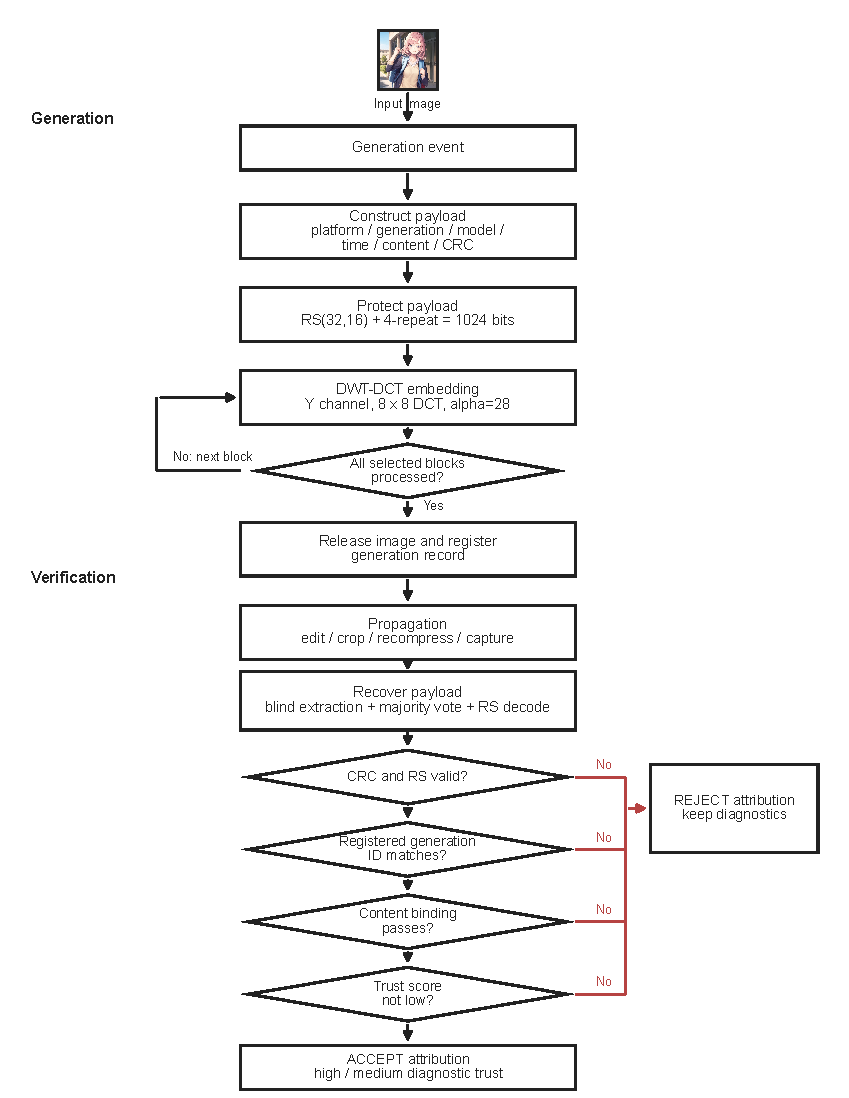
\includegraphics[width=0.98\linewidth]{fig1_framework.pdf}
  \caption{End-to-end flowchart of generation-time registration and
  verification-time acceptance testing. A failed integrity, registry, or
  content-binding check prevents attribution, while the recovered fields and
  trust evidence remain available for diagnosis.}
  \label{fig:overview}
\end{figure}

The design addresses three different failure sources. Error-control coding
addresses corruption of the watermark channel, registry matching addresses a
valid-looking payload whose generation identifier is not registered, and
content binding addresses a payload that is valid but belongs to another
image. The weighted trust score is computed only after these checks and is
therefore not used as a substitute for any hard constraint. The following
subsections describe each stage in execution order.

\subsection{Structured Payload Encoding and Error Control}
For each generation event, the platform first builds the 128-bit payload
$P$ according to Eq.~\eqref{eq:payload-layout}. CRC-16 detects errors that
remain after image-domain extraction and error correction. The 16-byte payload
is then encoded with the shortened Reed--Solomon code RS(32,16), producing a
32-byte codeword that can correct up to eight erroneous bytes in this
configuration. Error-controlled watermark payloads have previously been used
for robust data provenance \cite{saberi_drew_2024}; here the code protects a
structured generation record rather than an unstructured message.

Let $\Phi_{\mathrm{b}}(\cdot)$ convert bytes to bits and let
$\mathcal{M}_4(\cdot)$ denote fourfold repetition. The transmitted bit sequence
is
\begin{equation}
  \mathbf{b}
  =\mathcal{M}_4\!\left(
    \Phi_{\mathrm{b}}\!\left(
      \operatorname{RS}_{32,16}(P)
    \right)
  \right),
  \qquad
  |\mathbf{b}|=32\times8\times4=1024.
  \label{eq:coded-payload}
\end{equation}
Thus, every bit of the RS codeword occupies four adjacent positions of
$\mathbf{b}$. No additional interleaver is used in the current
implementation. The redundancy factor is eight relative to the 128-bit
payload: RS adds 16 parity bytes and repetition expands every byte-level bit
four times.

During decoding, the four copies of each RS bit are first combined by majority
vote. The resulting 256-bit sequence is byte-aligned and passed to the RS
decoder. If RS decoding succeeds, CRC-16 is recomputed over the 14-byte header.
The integrity event is
\begin{equation}
  I_{\mathrm{int}}
  =I_{\mathrm{RS}}\wedge I_{\mathrm{CRC}},
  \label{eq:integrity-gate}
\end{equation}
where $I_{\mathrm{RS}}$ and $I_{\mathrm{CRC}}$ are binary success indicators.
A failure of either indicator prevents subsequent evidence from being treated
as a valid registered payload, although the partially decoded fields remain
available for diagnostics. Figure~\ref{fig:payload} shows the bit allocation
and coding expansion.

\begin{figure}[!htbp]
  \centering
  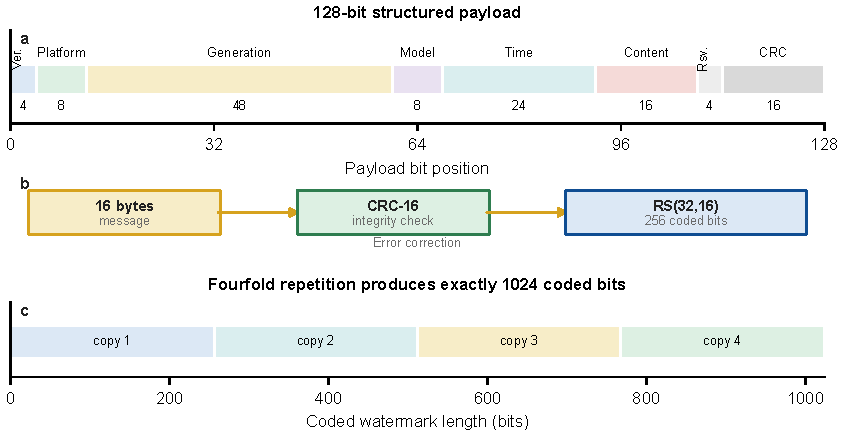
\includegraphics[width=\linewidth]{fig2_payload_ecc.pdf}
  \caption{Structured 128-bit payload and its expansion through CRC-16,
  RS(32,16), and fourfold repetition coding.}
  \label{fig:payload}
\end{figure}

\subsection{DWT--DCT Blind Embedding and Extraction}
The watermark is embedded after image generation and is therefore independent
of a particular generator architecture. We convert $X$ from RGB to YCrCb and
operate only on the luminance component $Y$. A one-level Haar DWT produces an
approximation band $A$ with one quarter of the spatial resolution. For a
$512\times512$ image, $A$ has size $256\times256$ and is partitioned into
$32\times32$ non-overlapping $8\times8$ blocks, giving exactly 1024 blocks for
the 1024 coded bits. DWT and DCT have complementary roles: the wavelet
decomposition isolates a lower-frequency representation, while the block DCT
concentrates local energy and provides a compact coefficient pair for
differential embedding. Related differential DWT--DCT designs exploit
coefficient relationships for blind extraction
\cite{benoraira_blind_2015,najafi_robust_2017}.

For block $j$, let $C_j(u,v)$ be the 8-by-8 DCT coefficient at vertical index
$u$ and horizontal index $v$, and define the carrier
\begin{equation}
  \Delta_j=C_j(3,2)-C_j(2,3).
  \label{eq:carrier-difference}
\end{equation}
For bit $b_j\in\{0,1\}$ and embedding strength $\alpha>0$, the target
difference is
\begin{equation}
  \tau_j=\alpha(2b_j-1).
  \label{eq:target-difference}
\end{equation}
We move the two coefficients by half the required gap:
\begin{equation}
\begin{aligned}
  \delta_j&=\frac{\tau_j-\Delta_j}{2},\\
  \tilde{C}_j(3,2)&=C_j(3,2)+\delta_j,\\
  \tilde{C}_j(2,3)&=C_j(2,3)-\delta_j.
\end{aligned}
  \label{eq:coefficient-update}
\end{equation}
Consequently,
\begin{equation}
  \tilde{C}_j(3,2)-\tilde{C}_j(2,3)=\tau_j,
  \label{eq:embedded-difference}
\end{equation}
and blind extraction requires only
\begin{equation}
  \hat{b}_j=
  \begin{cases}
    1, & \tilde{C}_j(3,2)-\tilde{C}_j(2,3)>0,\\
    0, & \text{otherwise}.
  \end{cases}
  \label{eq:blind-extraction}
\end{equation}
No original image or reference watermark is needed at extraction time.

The assignment of payload positions to spatial blocks is controlled by a
seeded permutation $\pi_\kappa$ of $\{1,\ldots,1024\}$, where
$\kappa=20260910$ in the reported configuration. The permutation decorrelates
the payload order from the raster order of image blocks. It is a
reproducibility and layout mechanism, not a claim of cryptographic secrecy.
After all selected blocks are updated, the inverse block DCT, inverse Haar DWT,
clipping, and YCrCb-to-RGB conversion produce the released image $Y$.
Figure~\ref{fig:dwt-dct} illustrates the embedding and extraction path. The
current instantiation uses $\alpha=28$; the quality--robustness tradeoff of
this choice is evaluated experimentally rather than assumed here.
Table~\ref{tab:parameters} summarizes the embedding and verification settings.

\begin{figure}[!htbp]
  \centering
  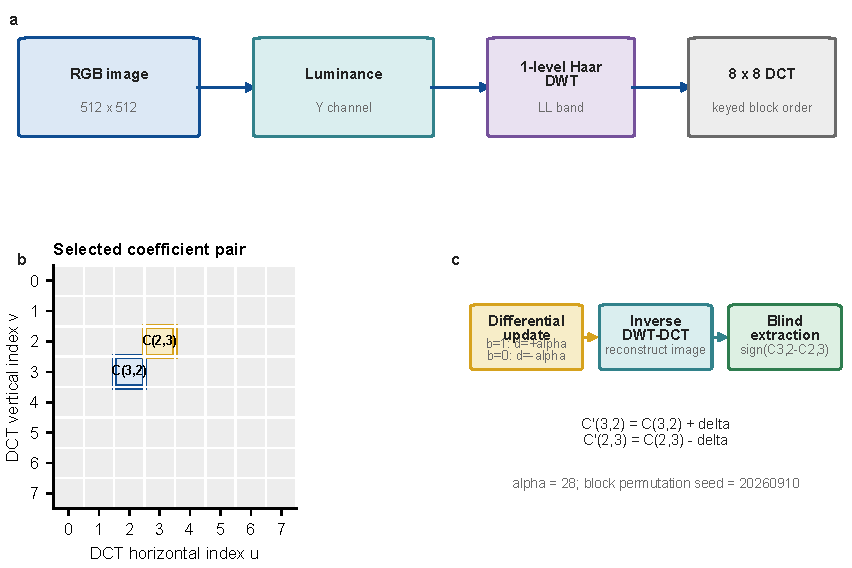
\includegraphics[width=\linewidth]{fig3_dwt_dct.pdf}
  \caption{DWT--DCT embedding and blind extraction on the luminance channel.
  The enlarged 8 x 8 coefficient map identifies the selected pair
  $C(3,2)$ and $C(2,3)$.}
  \label{fig:dwt-dct}
\end{figure}

\subsection{Multi-Field Database Verification}
Each registry record $R_i$ contains the original platform and model strings,
generation identifier, timestamp, full content SHA-256 digest, and the
corresponding payload-field projections. It also stores image descriptors used
for candidate evidence and content binding. For a decoded payload
$\hat{P}$, five binary checks are performed against record $R_i$:
\begin{enumerate}
  \item the recovered generation projection equals the registry projection;
  \item the recovered platform projection equals the registry projection;
  \item the recovered model-version projection equals the registry projection;
  \item the recovered timestamp differs from the registered timestamp by no
        more than 24 hours; and
  \item the recovered content projection equals the registry content
        projection.
\end{enumerate}
The field-consistency score is the fraction of satisfied checks,
\begin{equation}
  F_i=\frac{1}{5}\sum_{k=1}^{5}
  \mathbf{1}\!\left[\text{check}_k(\hat{P},R_i)\text{ is true}\right].
  \label{eq:field-score}
\end{equation}

To provide a continuous content cue before the stronger binding check, we
compute a 64-bit average hash by converting the query to grayscale, resizing it
to $8\times8$, thresholding each pixel against the mean, and flattening the
binary map. With bitwise Hamming similarity $H_i\in[0,1]$, the candidate score
for record $R_i$ is
\begin{equation}
  Q_i=0.45F_i+0.25H_i+0.30G_i,
  \label{eq:candidate-score}
\end{equation}
where $G_i\in\{0,1\}$ indicates an exact recovered-generation match.
Perceptual hashing provides compact image comparability under recompression
and moderate resizing \cite{sharma_distance_2024,wang_perceptual_2021}, but it
is used here only as one component of candidate evidence.

Candidates are ordered lexicographically by $(G_i,Q_i)$. This ensures that a
content-binding test is performed against the record whose generation
identifier was actually recovered rather than against an unrelated record with
a slightly higher weighted score. The current implementation scans all
registry records; approximate-nearest-neighbour indexing and distributed
registry search are outside the scope of this manuscript. The highest-ranked
record is retained even when its generation identifier does not match, because
the resulting fields support failure diagnosis.

\subsection{Content Binding and Flat-Image Fallback}
Registry consistency alone cannot distinguish a genuine image from a
different image carrying a copied but otherwise valid payload. We therefore
compare the query $Q$ with the registered source image associated with the
selected record. Oriented FAST and rotated BRIEF (ORB)
\cite{rublee_orb_2011} extracts at most 800 keypoints with FAST threshold 10
and stores 256-bit binary descriptors. A brute-force Hamming matcher obtains
the first and second nearest descriptors for each query point. A match is
counted when
\begin{equation}
  d_1\le 32
  \quad\text{or}\quad
  d_1<0.75d_2,
  \label{eq:orb-match-rule}
\end{equation}
where $d_1$ and $d_2$ are the nearest and second-nearest descriptor distances.
If $m$ matches are obtained, the ORB binding score is
\begin{equation}
  B_{\mathrm{ORB}}
  =\frac{m}{\max\!\left(1,\min(N_q,N_r)\right)},
  \label{eq:orb-score}
\end{equation}
where $N_q$ and $N_r$ are the query and registry keypoint counts.

Highly uniform images may not provide ten keypoints on either side, in which
case ORB scores are unreliable. For this condition, we construct an
$8\times8$ RGB layout signature by quantizing each colour value to 16 levels
and compute
\begin{equation}
  B_{\mathrm{flat}}
  =\frac{1}{2}H_{\mathrm{avg}}
  +\frac{1}{2}\left(1-\frac{1}{15}\mathbb{E}|q-r|\right),
  \label{eq:flat-score}
\end{equation}
where $q$ and $r$ are the query and reference quantized colour values and
$H_{\mathrm{avg}}$ is the average-hash similarity. The fallback uses threshold
$\tau_{\mathrm{flat}}=0.90$; the ORB path uses
$\tau_{\mathrm{ORB}}=0.30$. The content-binding decision is
\begin{equation}
  B(Q,R_{i^*})=
  \begin{cases}
    B_{\mathrm{flat}}\ge\tau_{\mathrm{flat}}, & \text{fallback path},\\
    B_{\mathrm{ORB}}\ge\tau_{\mathrm{ORB}}, & \text{otherwise}.
  \end{cases}
  \label{eq:content-binding-gate}
\end{equation}
The conservative flat-image threshold reflects the ambiguity of colour/layout
signatures on low-texture inputs; its behaviour is reported as a targeted
stress test in the experiments.

\subsection{Trust Scoring and Calibration}
After a registry record has been selected and content binding has been
evaluated, the joint trust score combines integrity, registry consistency,
perceptual similarity, and exact generation matching:
\begin{equation}
  S
  =0.25I_{\mathrm{CRC}}
  +0.20I_{\mathrm{RS}}
  +0.30F_{i^*}
  +0.15H_{i^*}
  +0.10G_{i^*}.
  \label{eq:trust-score}
\end{equation}
The score is mapped to three levels using
\begin{equation}
  \ell(S)=
  \begin{cases}
    \text{high}, & S\ge0.55,\\
    \text{medium}, & 0.32\le S<0.55,\\
    \text{low}, & S<0.32.
  \end{cases}
  \label{eq:trust-levels}
\end{equation}

The trust score is not itself the acceptance rule. Final acceptance is
\begin{equation}
  a=
  I_{\mathrm{CRC}}
  \wedge I_{\mathrm{RS}}
  \wedge G_{i^*}
  \wedge \mathbf{1}[S\ge0.32]
  \wedge B(Q,R_{i^*}),
  \label{eq:acceptance}
\end{equation}
so a high scalar score cannot override a failed integrity check, an
unregistered generation identifier, or a content mismatch. The thresholds
0.55 and 0.32 are operational cutoffs selected from an image-disjoint
calibration split; calibration results and held-out rates are reported in the
experiments, rather than interpreted as deployment probabilities. Consequently,
a format-valid but unregistered payload can retain a medium or high diagnostic
score while still being rejected because $G_{i^*}=0$.

\subsection{Alignment Search and Verification Procedure}
Cropping and rescaling can remove or displace watermark blocks even when the
payload itself remains present. The verifier therefore evaluates an identity
candidate and a deterministic set of spatial hypotheses. The downscaling
factors are
\begin{equation}
  \mathcal{S}_{\mathrm{align}}
  =\{0.80,0.85,0.875,0.90,0.925,0.95\}.
  \label{eq:alignment-scales}
\end{equation}
Each downscaled candidate is padded back to the original dimensions using
either edge replication or reflection. For scale $1.05$, the enlarged image is
centre-cropped back to the original dimensions. These choices yield 14
alignment candidates for the reported $512\times512$ setting.

For each candidate $A_r(Q)$, the verifier extracts 1024 bits, performs
majority and RS decoding, computes $F_i$, $H_i$, $Q_i$, and $G_i$ for the
registry, applies the content-binding gate, and evaluates
Eq.~\eqref{eq:acceptance}. The candidate with the highest trust score is
retained. To avoid unnecessary evaluations after an unambiguous result, the
search terminates early when a candidate satisfies the full acceptance rule,
matches the generation identifier, reaches high trust, and passes content
binding; otherwise all remaining candidates are evaluated and the
highest-scoring result is returned. Figure~\ref{fig:verification} shows the
separation between hard gates and graded trust.

\begin{figure}[!htbp]
  \centering
  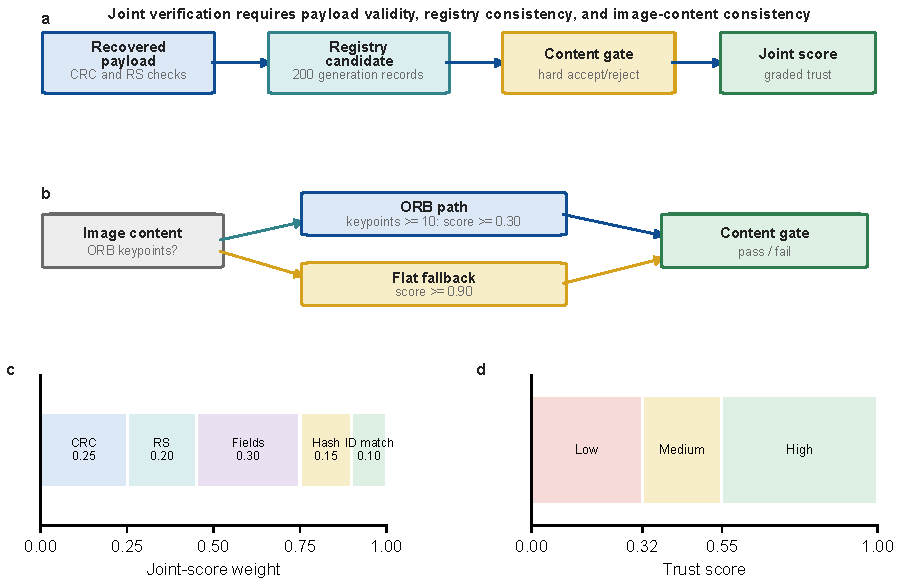
\includegraphics[width=\linewidth]{fig4_verification.pdf}
  \caption{Joint verification architecture. The content-binding hard gate is
  separated from the weighted trust score, and the final score is mapped to
  low, medium, or high trust.}
  \label{fig:verification}
\end{figure}

The complete verifier is deterministic for a fixed image, registry, seed, and
configuration. Its output includes the alignment selected, recovered and
matched identifier projections, field-consistency score, average-hash
similarity, content-binding score and method, trust score, trust level, and
final decision. This diagnostic record supports failure attribution and makes
the relationship between a rejected image and the first unmet stage explicit.
\begin{table}[t]
\centering
\caption{Embedding, error-control, and verification parameters.}
\label{tab:parameters}
\begin{tabular}{l l}
\toprule
Parameter & Value \\
\midrule
Input size & 512 x 512 px \\
Color/luminance domain & Y channel \\
DWT & Haar, level 1 \\
DCT block & 8 x 8 \\
Coefficient pair & (3,2) and (2,3) \\
Embedding strength & alpha = 28 \\
Block selection seed & 20260910 \\
Error control & RS(32,16) + 4-repeat \\
Coded payload length & 1024 bits \\
ORB binding threshold & 0.30 \\
Flat-image fallback & 0.90 \\
Medium trust threshold & 0.32 \\
High trust threshold & 0.55 \\
\bottomrule
\end{tabular}
\end{table}


\section{Experiments}\label{sec:experiments}

\subsection{Dataset and Implementation}
The evaluation benchmark contained 300 images at $512\times512$ pixels. The
200 registered positives were generated with Stable Diffusion 1.5 using the
Anything V5 checkpoint, with 25 images in each of eight prompt categories
(landscape, portrait, city, object, animal, food, fantasy, and abstract). The
negative set contained 50 images generated by Elysium Anime V3 and 50 natural
images from Wikimedia Commons. The natural images were converted by
short-side resizing followed by centre cropping; source dimensions, crop
coordinates, output hashes, and licence metadata were retained. All 300 files
had distinct SHA-256 digests. Table~\ref{tab:dataset} summarises the benchmark.
\begin{table}[t]
\centering
\caption{Composition of the 300-image evaluation benchmark.}
\label{tab:dataset}
\begin{tabular}{l l r l}
\toprule
Group & Source & Count & Role \\
\midrule
Platform positive & SD 1.5 / Anything V5 & 200 & Registered provenance records \\
Other-model AI negative & Elysium Anime V3 & 50 & Non-platform AI images \\
Natural negative & Wikimedia Commons & 50 & Non-AI images \\
\bottomrule
\end{tabular}
\par\smallskip
\footnotesize All images were evaluated at 512 x 512. Natural-image licenses: CC BY 1.0 (1), CC BY 2.0 (1), CC BY 3.0 (1), CC BY 4.0 (2), CC BY-SA 2.0 (2), CC BY-SA 3.0 (7), CC BY-SA 4.0 (31), CC0 (4), FAL (1).
\end{table}


The embedding and verification implementation used Python 3.13.1, NumPy 2.1.3,
OpenCV 4.11.0, PyWavelets 1.8.0, \texttt{reedsolo} 1.7.0, and Pillow 12.3.0.
Image generation was performed through the local Stable Diffusion WebUI on an
NVIDIA GeForce RTX 4050 Laptop GPU. The watermarking and verification
experiments were executed on an Intel Core i5-13500H host with 32 GB of memory.
The carrier contains no trainable parameters. The block-permutation and attack
seed was 20260910; the image-disjoint calibration split used seed 20261028.
Unless stated otherwise, carrier and coding results use $\alpha=28$.

Each registered positive was evaluated under 13 single transformations, six
compound transformations, and two stronger propagation simulators, for 21
conditions with $n=200$ each. The transformations included JPEG compression,
resizing, centre cropping, Gaussian and salt-and-pepper noise,
brightness/contrast adjustment, Gaussian blur, and a light screenshot
simulation. Compound conditions combined cropping or resizing with JPEG
compression, blur, or noise. The screen-capture simulator added scaling,
perspective, moir\'e, colour shift, blur, noise, and recompression; the
print--scan simulator additionally modelled paper texture, yellowing, ink blur,
gamma shift, and scanner noise. Following common robustness reporting practice
\cite{an_waves_2024}, we report acceptance rate, mean bit error rate (BER), and
Wilson 95\% confidence intervals. Acceptance is the binary decision in
Eq.~\eqref{eq:acceptance}; BER is measured before error correction by comparing
the 1024 extracted and embedded bits.

\subsection{Image Quality}
The final configuration preserved image fidelity over the 200 registered
images. The mean PSNR was 39.65 dB, the median was 39.87 dB, and the
5th--95th percentile range was 36.60--42.23 dB. The minimum was 30.28 dB in the
abstract-image category, whose mean PSNR was 37.82 dB; all other category means
were between 38.70 and 40.73 dB. SSIM averaged 0.998980, with a median of
0.999167 and a minimum of 0.995417.

Figure~\ref{fig:watermark-example} shows the median-PSNR image, global and
10-fold-amplified residual views, and the full PSNR/SSIM distributions. The
residual reveals a spatially distributed embedding pattern, while the
published image preserves the original appearance at the displayed scale. The
distribution is also relevant for deployment: lower-tail images, rather than
only the representative example, determine whether a fixed embedding strength
is acceptable.

\begin{figure}
  \centering
  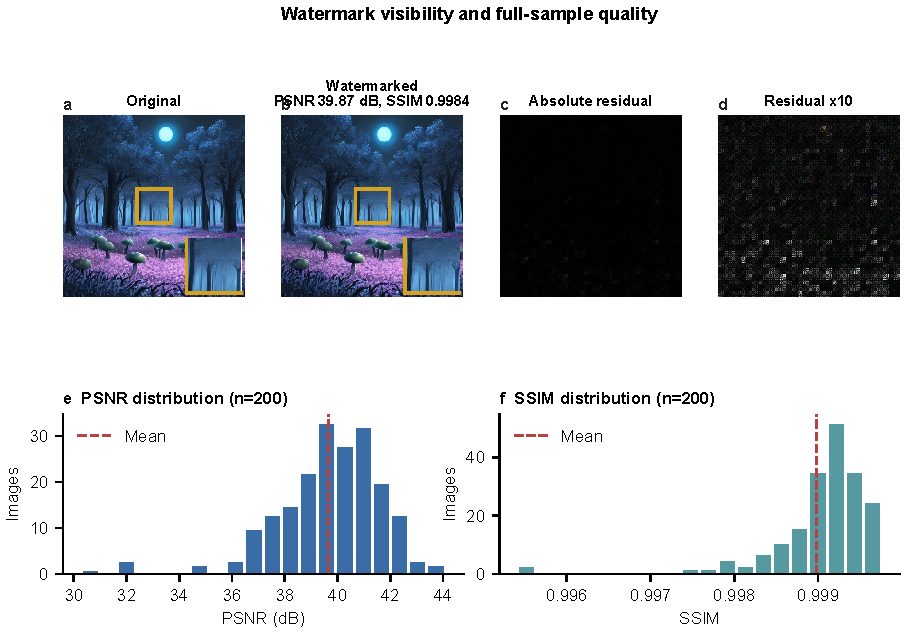
\includegraphics[width=\linewidth]{fig5_watermark_example.pdf}
  \caption{Watermark visibility for the median-PSNR image with enlarged centre
  patches, together with the PSNR and SSIM distributions over all $n=200$
  registered positives.}
  \label{fig:watermark-example}
\end{figure}

\subsection{Robustness Under Image Transformations}
Verification was stable under compression, resizing, and additive
perturbations. Clean images and JPEG Q90 achieved 100\% acceptance; JPEG Q50 and
Q70, resize by 0.75, and Gaussian noise with $\sigma=8$ each achieved 99.5\%.
The light screenshot simulation and salt-and-pepper noise achieved 99.5\% each.
Brightness/contrast adjustment and Gaussian blur produced
96.0\% and 98.0\% acceptance. Centre cropping to 90\% of the original side
length followed by resizing back to $512\times512$ was the hardest standard
single operation, with 92.0\% acceptance and a mean BER of 0.0850.

Compound propagation reduced performance further when geometric and compression
effects were combined. Crop0.9+JPEG70 achieved 87.5\% acceptance, whereas
crop0.9+resize0.8+JPEG70 achieved 81.5\%; these conditions had mean BERs of
0.0918 and 0.0956. Resize+JPEG, screenshot+noise, blur+JPEG, and social
recompression achieved 99.5\%, 99.5\%, 96.0\%, and 99.5\%, respectively. The
same pattern is visible in Fig.~\ref{fig:robustness}, and Table~\ref{tab:robustness}
reports all 19 standard conditions.

The stronger propagation simulators exposed a clear boundary. Screen-capture
and print--scan simulation each produced 0/200 accepted images, with mean BERs
of 0.535 and 0.495. These observations indicate loss of payload recovery under
the tested geometric and acquisition models; they do not establish failure
rates for arbitrary cameras, displays, printers, or scanners. Table~\ref{tab:calibration-negative}
reports these stress tests separately from the lighter screenshot simulation.

\begin{figure}
  \centering
  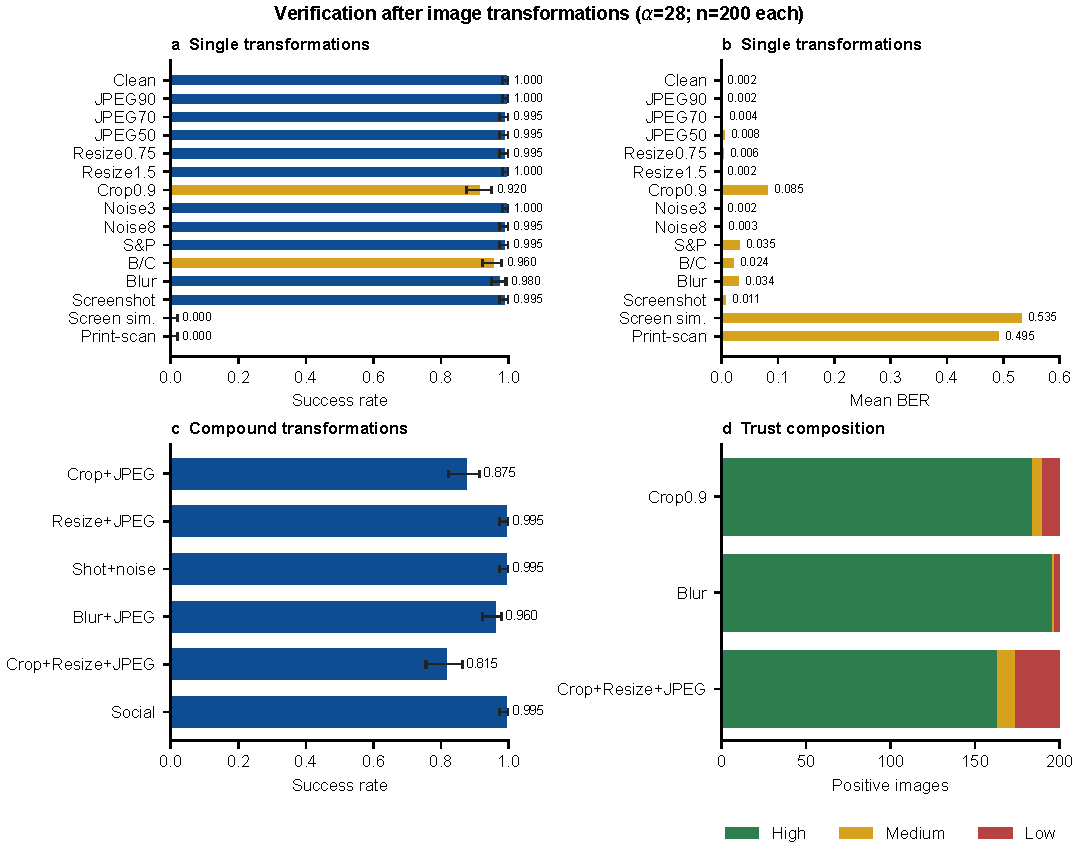
\includegraphics[width=\linewidth]{fig6_robustness.pdf}
  \caption{Verification success and mean BER under single and compound image
  transformations ($n=200$ per operation). Error bars show Wilson 95\%
  confidence intervals.}
  \label{fig:robustness}
\end{figure}
\begin{table}[t]
\centering
\caption{Verification success, mean BER, and trust composition under single and compound transformations.}
\label{tab:robustness}
\begin{tabular}{l l r r r}
\toprule
Family & Operation & N & Success (\%) & BER \\
\midrule
Single & Clean & 200 & 100.0 & 0.002 \\
Single & JPEG Q50 & 200 & 99.5 & 0.008 \\
Single & JPEG Q70 & 200 & 99.5 & 0.004 \\
Single & JPEG Q90 & 200 & 100.0 & 0.002 \\
Single & Resize x0.75 & 200 & 99.5 & 0.006 \\
Single & Resize x1.5 & 200 & 100.0 & 0.002 \\
Single & Crop 0.9 & 200 & 92.0 & 0.085 \\
Single & Gaussian noise sigma=3 & 200 & 100.0 & 0.002 \\
Single & Gaussian noise sigma=8 & 200 & 99.5 & 0.003 \\
Single & Salt-and-pepper 0.002 & 200 & 99.5 & 0.035 \\
Single & Brightness/contrast & 200 & 96.0 & 0.024 \\
Single & Gaussian blur 3x3 & 200 & 98.0 & 0.034 \\
Single & Screenshot simulation & 200 & 99.5 & 0.011 \\
Compound & Crop 0.9 + JPEG Q70 & 200 & 87.5 & 0.092 \\
Compound & Resize x0.75 + JPEG Q70 & 200 & 99.5 & 0.011 \\
Compound & Screenshot + noise sigma=3 & 200 & 99.5 & 0.012 \\
Compound & Blur + JPEG Q70 & 200 & 96.0 & 0.041 \\
Compound & Crop 0.9 + resize x0.8 + JPEG Q70 & 200 & 81.5 & 0.096 \\
Compound & Social recompression & 200 & 99.5 & 0.008 \\
\bottomrule
\end{tabular}
\par\smallskip
\footnotesize Each operation uses 200 registered positives. Success requires a valid CRC/RS decode, a database generation match, content binding, and a non-low trust score. Trust-level composition is shown in Fig. 6.
\end{table}


\subsection{Ablation Studies}
The carrier comparison revealed a quality--robustness tradeoff rather than
uniform superiority of DWT--DCT. DCT-only achieved 43.46 dB PSNR and matched or
exceeded DWT--DCT on the reported single operations, including 92.0\% crop
acceptance. DWT-only reduced crop acceptance to 39.0\%, while LSB embedding
failed every non-clean condition despite a 52.36 dB PSNR. Under compound
propagation, however, DWT--DCT retained 96.0\% acceptance for blur+JPEG70,
compared with 29.5\% for DCT-only. DCT-only was slightly stronger on
crop+JPEG70 and crop+resize+JPEG70. These results support retaining DWT--DCT
for the combined blur/compression condition without describing it as globally
more robust than DCT-only.

The coding ablation showed that both error-control layers contributed.
RS(32,16)+fourfold repetition achieved 92.0\% on crop0.9, compared with 81.5\%
for repetition without RS and 0.0\% for RS without repetition. The PSNR
difference between RS+repeat and repeat-only was only 0.03 dB. Raw payload
transmission fell to 52.5\% under JPEG50 and 0.0\% under cropping, showing that
the coded length is operationally necessary rather than merely redundant.

Embedding strength controlled the fidelity--robustness tradeoff. Increasing
$\alpha$ from 8 to 28 reduced mean PSNR from 40.72 to 39.65 dB, while JPEG50
acceptance rose from 1.0\% to 99.5\%, crop acceptance from 61.0\% to 92.0\%, and
blur acceptance from 23.0\% to 98.0\%. The improvement from $\alpha=24$ to
$\alpha=28$ was concentrated in the harder conditions: crop increased from
89.0\% to 92.0\% and blur from 96.5\% to 98.0\%, at a cost of approximately
0.31 dB PSNR. Figure~\ref{fig:ablation} and Table~\ref{tab:ablation} report the
14 carrier, coding, and strength configurations; the three verification modes
complete the 17-configuration set.

The three verification modes produced identical positive-set rates, so
registered positives alone do not isolate their security roles. The forged
payload and copied-watermark tests in Section~\ref{sec:security} provide that
evidence: watermark-only verification accepts a correctly formatted but
unregistered payload, whereas the joint mode rejects it, and enabling content
binding rejects a payload transplanted onto different image content.

\begin{figure}
  \centering
  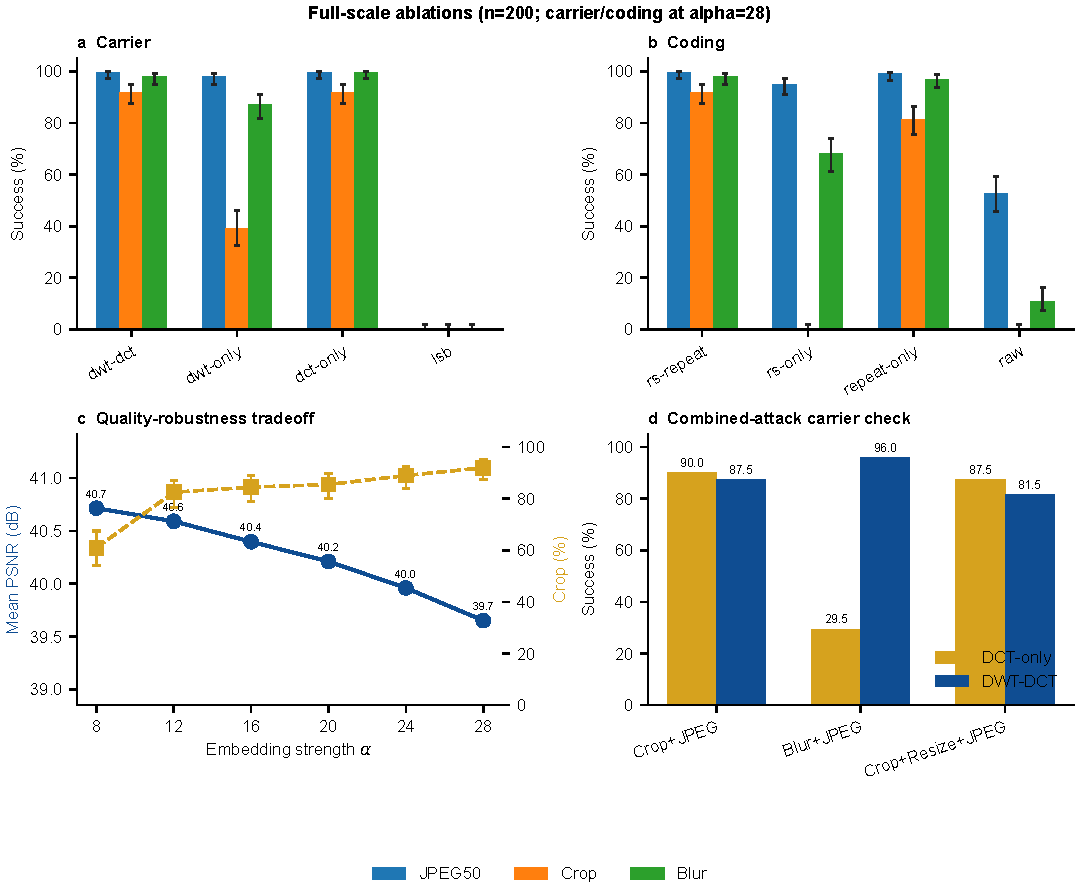
\includegraphics[width=\linewidth]{fig7_ablation.pdf}
  \caption{Full-scale carrier, coding, and embedding-strength ablations
  ($n=200$). Carrier and coding comparisons use $\alpha=28$. The final panel
  contrasts DCT-only and DWT--DCT under compound attacks.}
  \label{fig:ablation}
\end{figure}
\begin{table}[t]
\centering
\caption{Carrier, coding, and embedding-strength ablations.}
\label{tab:ablation}
\begin{tabular}{l l r r r r r r}
\toprule
Group & Configuration & PSNR (dB) & SSIM & JPEG50 (\%) & Crop (\%) & Blur (\%) & Screenshot (\%) \\
\midrule
carrier & dwt\_dct & 39.65 & 0.9990 & 99.5 & 92.0 & 98.0 & 99.5 \\
carrier & dwt\_only & 41.36 & 0.9994 & 98.0 & 39.0 & 87.0 & 99.5 \\
carrier & dct\_only & 43.46 & 0.9996 & 99.5 & 92.0 & 99.5 & 100.0 \\
carrier & lsb & 52.36 & 1.0000 & 0.0 & 0.0 & 0.0 & 0.0 \\
coding & rs\_repeat & 39.65 & 0.9990 & 99.5 & 92.0 & 98.0 & 99.5 \\
coding & rs\_only & 44.22 & 0.9997 & 95.0 & 0.0 & 68.0 & 94.5 \\
coding & repeat\_only & 39.62 & 0.9990 & 99.0 & 81.5 & 97.0 & 98.5 \\
coding & raw & 45.92 & 0.9998 & 52.5 & 0.0 & 11.0 & 47.5 \\
alpha & alpha\_8 & 40.72 & 0.9992 & 1.0 & 61.0 & 23.0 & 60.0 \\
alpha & alpha\_12 & 40.59 & 0.9992 & 44.5 & 82.5 & 64.5 & 92.0 \\
alpha & alpha\_16 & 40.40 & 0.9991 & 98.5 & 84.5 & 83.0 & 97.0 \\
alpha & alpha\_20 & 40.21 & 0.9991 & 99.5 & 85.5 & 91.5 & 98.5 \\
alpha & alpha\_24 & 39.96 & 0.9990 & 99.5 & 89.0 & 96.5 & 99.5 \\
alpha & alpha\_28 & 39.65 & 0.9990 & 99.5 & 92.0 & 98.0 & 99.5 \\
\bottomrule
\end{tabular}
\par\smallskip
\footnotesize The ablation uses 200 positive images and alpha=28 for carrier and coding comparisons.
\end{table}


\subsection{Low-False-Positive Calibration}
Calibration and evaluation were separated by image to prevent repeated attack
variants of the same source from appearing on both sides. The calibration and
held-out halves each contained 100 positive and 50 negative images. With 19
attack variants per image, each half produced 1,900 positive and 950 negative
score observations. Positive strata were balanced across the eight prompt
categories, and each half received 25 natural and 25 other-model negatives.
The area under the ROC curve was 0.998693 on the calibration half and 0.999833
on the held-out half. Cluster-bootstrap intervals over 2,000 image-level
resamples were 0.996138--0.999970 and 0.999570--1.000000, respectively.

The retained operational thresholds also transferred to held-out images.
At the high-trust cutoff of 0.55, held-out TPR was 97.3\% with an observed FPR
of 0.00\%. At the medium-or-higher cutoff of 0.32, held-out TPR was 98.0\% with
an observed FPR of 0.32\%. A target-FPR calibration point of 0.01 selected a
threshold of 0.310 on the calibration half and transferred to an observed
0.53\% FPR and 98.0\% TPR on the held-out half. These finite-sample observations
are reported as operating characteristics; an empirical zero does not establish
a population FPR of zero. Figure~\ref{fig:calibration} shows the ROC curves and
the held-out score distributions.

\begin{figure}
  \centering
  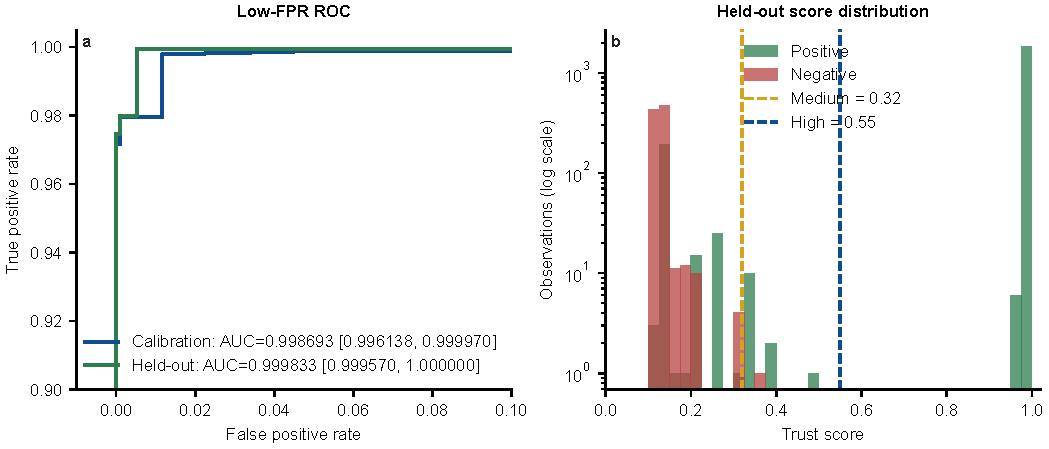
\includegraphics[width=\linewidth]{fig8_calibration.pdf}
  \caption{Calibration and held-out ROC curves and held-out trust-score
  distributions. The split is by image; AUC intervals use cluster
  bootstrapping over images.}
  \label{fig:calibration}
\end{figure}

\subsection{Comparison with External Watermarking Methods}
External comparisons used the 50 positive images for which every method
produced a result. The DWT--DCT and DWT--DCT--SVD implementations from
\texttt{invisible-watermark} received the same 1024 coded bits as the proposed
carrier. RivaGAN was evaluated with its native 32-bit payload and is therefore a
short-payload robustness reference rather than an equal-payload baseline.

The proposed method achieved 40.33 dB PSNR and 0.999302 SSIM on the matched
subset. It accepted 100\% of JPEG50, blur, and screenshot cases, 94\% of
crop0.9 cases, and 88\% of crop+resize+JPEG cases. External DWT--DCT did not
recover the 1024-bit payload in any reported condition, despite its high SSIM.
External DWT--DCT--SVD accepted 72\% under JPEG50 and 100\% under blur and
screenshot simulation, but 0\% under cropping and crop+resize+JPEG. RivaGAN
accepted 100\% in all five reported conditions at 40.48 dB PSNR, but its 32-bit
payload cannot carry the complete structured record and error-control
overhead used here. Table~\ref{tab:external} gives the matched results, while
Fig.~\ref{fig:external} reports success and BER with Wilson intervals.

Figure~\ref{fig:external-visual} compares representative landscape and portrait
images selected by median PSNR. The proposed method produced 41.10 dB/0.9994
for the landscape example and 39.80 dB/0.9994 for the portrait example.
The transform-domain baselines used lower PSNR on these examples, whereas
RivaGAN produced similar visual fidelity with its shorter payload. The examples
support visual plausibility only; the full-sample metrics and attack results
remain the quantitative evidence.

\begin{figure}
  \centering
  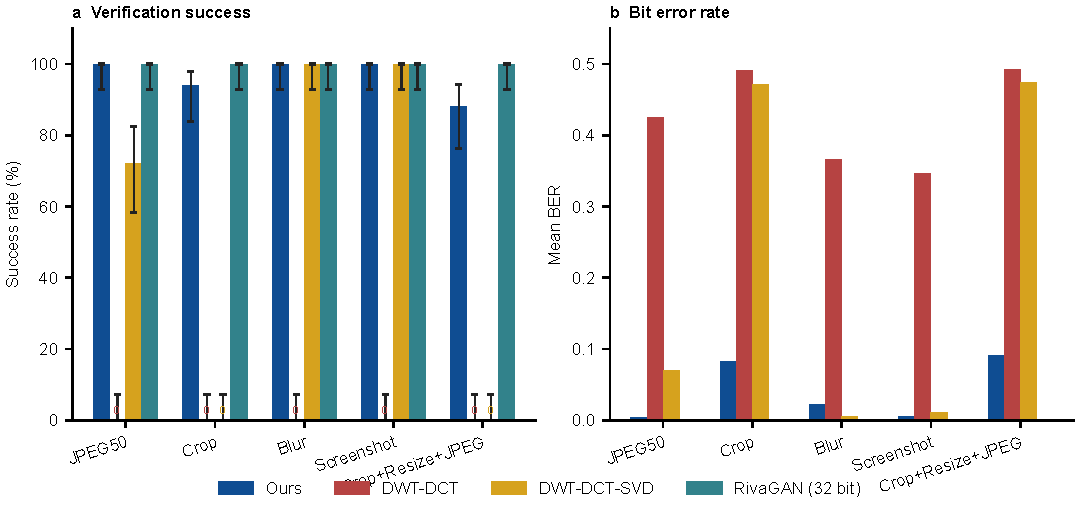
\includegraphics[width=\linewidth]{fig9_external.pdf}
  \caption{Comparison with external watermarking methods on the common
  50-image subset. Panel (a) reports verification success with Wilson 95\%
  confidence intervals; panel (b) reports mean BER.}
  \label{fig:external}
\end{figure}
\begin{figure}
  \centering
  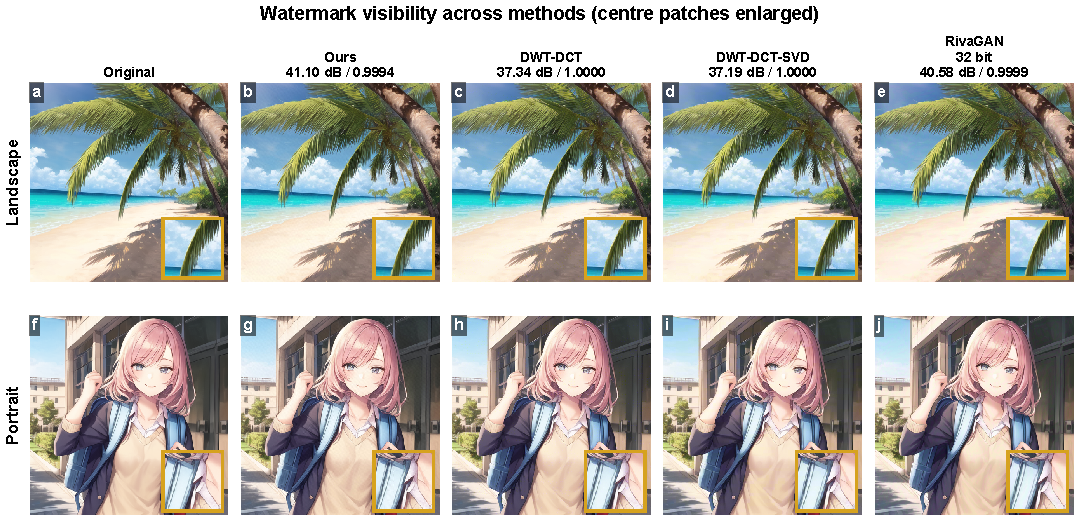
\includegraphics[width=\linewidth]{fig10_multimethod_visual.pdf}
  \caption{Visual comparison of watermarked landscape and portrait images.
  The insets enlarge the central patches. PSNR/SSIM values are shown above
  each column; RivaGAN carries a 32-bit payload.}
  \label{fig:external-visual}
\end{figure}
\begin{table}[t]
\centering
\caption{Comparison with external watermarking methods on the common 50-image subset.}
\label{tab:external}
\begin{tabular}{l r r r r}
\toprule
Metric & Ours & DWT-DCT & DWT-DCT-SVD & RivaGAN \\
\midrule
Payload bits & 1024 & 1024 & 1024 & 32 \\
N & 50 & 50 & 50 & 50 \\
PSNR (dB) & 40.33 & 37.76 & 37.68 & 40.48 \\
SSIM & 0.9993 & 1.0000 & 1.0000 & 0.9999 \\
JPEG50 (\%) & 100.0 & 0.0 & 72.0 & 100.0 \\
Crop (\%) & 94.0 & 0.0 & 0.0 & 100.0 \\
Blur (\%) & 100.0 & 0.0 & 100.0 & 100.0 \\
Screenshot (\%) & 100.0 & 0.0 & 100.0 & 100.0 \\
Crop+Resize+JPEG (\%) & 88.0 & 0.0 & 0.0 & 100.0 \\
\bottomrule
\end{tabular}
\par\smallskip
\footnotesize RivaGAN uses a native 32-bit payload and is a short-payload reference, not an equal-payload baseline.
\end{table}


\subsection{Security and Failure-Boundary Tests}
\label{sec:security}
The registry and content checks were evaluated with format-valid but invalid
payloads. Across 20 forged payloads whose generation identifiers were absent
from the registry, watermark-only verification accepted 20/20, whereas
database-only and joint verification accepted 0/20. The mean joint score was
0.640, but exact generation matching remained false, so the hard acceptance
condition prevented attribution. This result illustrates why the scalar trust
score must be reported separately from the final decision.

The transplanted-watermark test used 50 paired donor-target trials. With
content binding disabled, joint verification accepted all 50 copies; with
binding enabled, it accepted none. The copied trials had a mean
content-binding score of 0.0143, compared with 0.860 for JPEG70 positives,
0.893 for crop0.9 positives, and 0.905 for clean positives. The ORB gate
therefore separated the tested payload copies from legitimate processed
images. This result applies to the 50 paired trials and is not a full
$50\times50$ donor--target matrix.

Texture-poor images required a separate fallback. On 11 synthetic low-texture
images and 44 positive cases, the ordinary threshold of 0.30 produced 95.5\%
TPR but 100\% FPR. The fallback threshold of 0.90 reduced FPR to 0.00\% while
retaining 75.0\% TPR. This stress set is intentionally small and concentrated,
so the result supports the conservative fallback policy but not a general
estimate for all flat images.

Clean joint verification produced 0/100 false positives, and the six compound
attack conditions produced 0/600 false positives on negative observations.
The two strong propagation simulators remained systematic failures, with 0/200
accepted for both screen capture and print--scan. Table~\ref{tab:security} and
Table~\ref{tab:calibration-negative} collect the forgery, copy, flat-image,
negative, calibration, and stress-test outcomes.

Figure~\ref{fig:case-gallery} traces one registered image through clean, JPEG70,
crop0.9, and print--scan conditions. The first three versions were accepted
with high trust; the cropped case required a
\texttt{scale\_0.9\_reflect} alignment. The print--scan version was rejected
even though its content-binding score remained above the ORB threshold, showing
that payload loss and content mismatch are independent failure sources.

\begin{table}[t]
\centering
\caption{Forgery, copy attack, and flat-image security tests.}
\label{tab:security}
\begin{tabular}{>{\raggedright\arraybackslash}p{27mm} >{\raggedright\arraybackslash}p{32mm} >{\raggedright\arraybackslash}p{38mm} >{\raggedright\arraybackslash}p{48mm}}
\toprule
Test & Condition & Accepted / tested & Interpretation \\
\midrule
Forged valid payload & Watermark only & 20 / 20 & No registry/content rejection \\
Forged valid payload & Joint verification & 0 / 20 & Unregistered generation ID rejected \\
Copied watermark & Binding off & 50 / 50 & Payload-only verification is vulnerable \\
Copied watermark & Binding on & 0 / 50 & Content mismatch rejected \\
Flat-image fallback & Threshold 0.30 & TPR 95.5\%; FPR 100.0\% & Unsafe for flat images \\
Flat-image fallback & Threshold 0.90 & TPR 75.0\%; FPR 0.0\% & Conservative fallback \\
\bottomrule
\end{tabular}
\par\smallskip
\footnotesize Copy testing contains 50 paired donor-target trials. Flat-image testing contains 11 synthetic images.
\end{table}

\begin{table}[t]
\centering
\caption{Calibrated trust thresholds, clean negatives, and physical stress tests.}
\label{tab:calibration-negative}
\begin{tabular}{>{\raggedright\arraybackslash}p{27mm} >{\raggedright\arraybackslash}p{32mm} >{\raggedright\arraybackslash}p{38mm} >{\raggedright\arraybackslash}p{48mm}}
\toprule
Test & Condition & Accepted / tested & Interpretation \\
\midrule
Held-out trust & Score >= 0.55 & TPR 97.3\%; FPR 0.00\% & High-confidence operating point \\
Held-out trust & Score >= 0.32 & TPR 98.0\%; FPR 0.32\% & Medium-or-higher operating point \\
Clean negatives & Joint verification & 0 / 100 & No observed clean false positives \\
Physical stress & Screen-capture simulator & 0 / 200 & Current carrier fails \\
Physical stress & Print-scan simulator & 0 / 200 & Current carrier fails \\
\bottomrule
\end{tabular}
\par\smallskip
\footnotesize Held-out rates aggregate repeated attack observations from 50 held-out negative images. Physical stress tests use 200 registered positives.
\end{table}

\begin{figure}
  \centering
  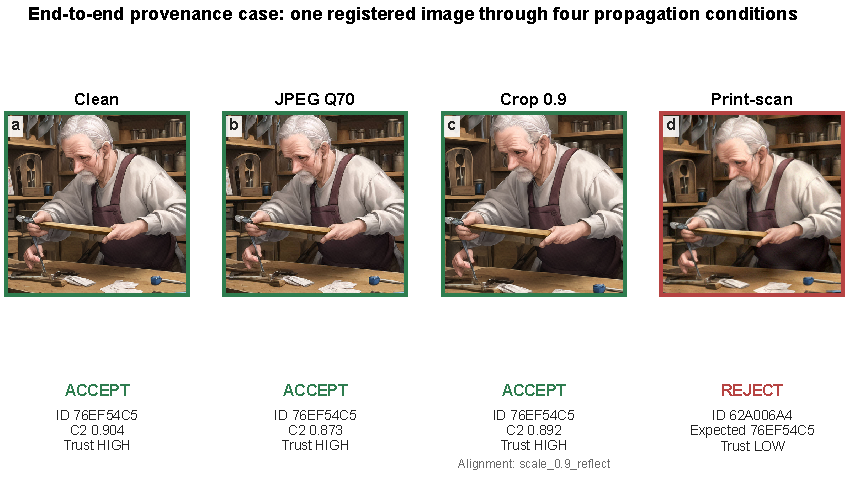
\includegraphics[width=\linewidth]{fig11_case_gallery.pdf}
  \caption{End-to-end verification of one registered image under clean,
  JPEG70, crop0.9, and print--scan propagation. C2 denotes the content-binding
  score. Green and red borders indicate final acceptance and rejection.}
  \label{fig:case-gallery}
\end{figure}

\subsection{Verification Failure Attribution}
\label{sec:failure-attribution}
To localize failures within the verification chain,
Fig.~\ref{fig:failure-attribution} replays each registered image under the same
21 single and compound propagation conditions and records the cumulative
outcome after CRC, RS decoding, generation-ID matching, exact field
consistency, content binding, and final trust acceptance. Across 4,200
sample--condition trajectories, 3,693 were accepted and 507 were rejected.
Every rejected trajectory first failed the payload-integrity stage; no
trajectory that recovered a valid CRC and RS codeword subsequently failed
registry matching, content binding, or the trust threshold. Rejection was
therefore dominated by an upstream recovery boundary rather than by
inconsistency in the later database checks. The largest observed losses were
8.0\% for crop0.9, 12.5\% for crop+JPEG70, 18.5\% for
crop+resize0.8+JPEG70, and 100\% for both the screen-capture and print--scan
stress simulators. These percentages describe the fixed 200-image evaluation
and the specified deterministic simulators; they are not estimates of failure
rates on arbitrary capture devices.

\begin{figure}
  \centering
  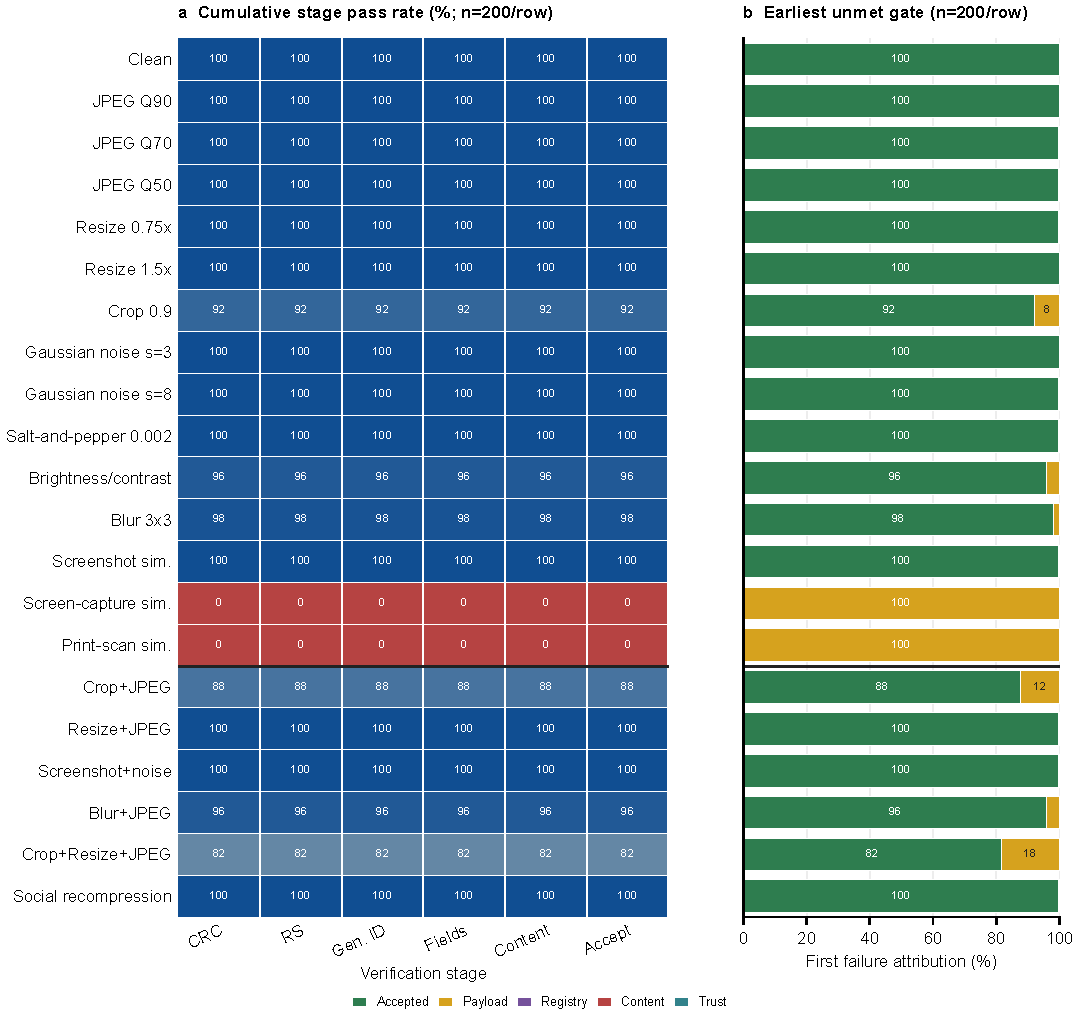
\includegraphics[width=\linewidth]{fig12_failure_attribution.pdf}
  \caption{Verification-stage failure attribution for 21 single and compound
  conditions ($n=200$ registered images per row). (a) Cumulative pass rate
  after CRC, RS decoding, generation-ID matching, exact field consistency,
  content binding, and final trust acceptance. (b) Earliest unmet gate. The
  accepted and rejected trajectories are mutually exclusive. ``Screenshot
  sim.'' is a light resize/JPEG simulation, whereas ``Screen-capture sim.'' and
  ``Print-scan sim.'' are stronger stress simulators and are not conflated
  with it.}
  \label{fig:failure-attribution}
\end{figure}

\section{Discussion}\label{sec:discussion}

\subsection{Interpretation}
The central result is not merely that a watermark survives several image
transformations. Rather, acceptance is conditioned jointly on payload
integrity, an exact registered-generation match, content binding, and non-low
trust. This distinction matters because a recovered watermark can be
syntactically valid without identifying a registered event or the image to
which it belongs. The forgery experiment isolates the first issue:
watermark-only verification accepted all 20 format-valid unregistered
payloads, whereas joint verification accepted none. The transplant experiment
isolates the second: with content binding disabled, all 50 copied payloads were
accepted; with binding enabled, none were accepted. The two mechanisms
therefore address different attacks and should not be reduced to a binary
watermark detector.

The failure-attribution experiment clarifies where the registered-positive
stress cases stop. All 507 rejected trajectories first failed payload
integrity, whereas no trajectory that recovered a valid CRC and RS codeword
subsequently failed registry matching, content binding, or the trust
threshold. This result explains the otherwise similar cumulative rows in
Fig.~\ref{fig:failure-attribution}: the later stages are not exercised unless
payload recovery succeeds. It also defines the role of the security tests.
Registered positives alone can measure recovery and false-negative behaviour;
forged and transplanted payloads are required to evaluate registry and
content-binding behaviour.

Cropping remains the hardest standard transformation because it removes image
area and displaces the keyed block layout. The 14-candidate alignment search
raised acceptance to 92.0\%, but repeated geometric processing still reduced
acceptance to 81.5\% for crop+resize+JPEG70 and 87.5\% for crop+JPEG70. The
stronger screen-capture and print--scan simulators produced no accepted image.
Because their failures also began at payload recovery, the observations are
consistent with residual geometric desynchronization and resampling rather
than inconsistency in the registry or content checks. The present evidence
does not identify which component of those simulators is dominant, and the
zero rates should not be extrapolated to physical devices without direct
capture experiments.

The carrier ablation shows that DWT--DCT is a design tradeoff rather than a
uniform improvement. DCT-only achieved higher PSNR and matched or exceeded
DWT--DCT on the reported single operations, including crop0.9. DWT--DCT
retained 96.0\% acceptance for blur+JPEG70, compared with 29.5\% for
DCT-only, which is the relevant reason for retaining it in the present
configuration. Likewise, RS and repetition improve different failure regions:
repetition supports local bit recovery, whereas RS becomes decisive when the
decoded codeword contains structured byte errors. These component results are
more informative than a single aggregate success rate.

The image-disjoint calibration supports using the trust score as a bounded
auxiliary signal. Held-out AUC was 0.999833, and the 0.32 operating point
produced 98.0\% TPR at an observed 0.32\% FPR. These rates do not make the
score a substitute for hard gates: a format-valid unregistered payload can
retain a high diagnostic score while still being rejected by the generation
matching condition. The reported zero FPR at 0.55 is an empirical observation
on the held-out sample, not evidence of zero population risk.

\subsection{Limitations}
The principal limitation is scope. The verifier is platform controlled: the
generation event, registry record, watermark configuration, and verification
logic are assumed to belong to a participating platform. It does not determine
whether an arbitrary image is AI-generated and does not establish attribution
across non-participating platforms. The benchmark contains 200 registered
images from one Stable Diffusion configuration, 50 images from another model,
and 50 natural images. It therefore measures behaviour on a controlled
benchmark rather than production traffic or a representative sample of
generators.

The attack evaluation is also simulator based. JPEG, resizing, cropping, noise,
blur, screenshot, screen capture, and print--scan are useful controlled stress
tests, but they do not reproduce every display, camera, printer, scanner, or
platform processing pipeline. The screen-capture and print--scan results are
therefore failure evidence for the current carrier, not deployment estimates.
The flat-image fallback contains only 11 synthetic low-texture images, and the
external comparison uses 50 images. RivaGAN has a native 32-bit payload and
serves as a short-payload reference rather than a fair long-payload competitor.

Two implementation boundaries also remain. The current registry is searched
exhaustively, so indexing cost and retrieval accuracy at production scale have
not been evaluated. The payload fields are truncated projections, and the
current construction has no cryptographic signature or secret-key
authentication. Registry trust is assumed. Larger registries, identifier
collisions, key management, compromised platforms, and long-term threshold
drift require separate analysis. The clean negative result of 0/100 should be
read with the corresponding finite-sample resolution.

\subsection{Deployment Implications}
In a controlled generation pipeline, the payload can serve as a compact
registry handle while the platform retains the full generation metadata.
Embedding should occur after the final generation step but before release, and
the released image, payload, and registry record should be committed as one
auditable event. The short watermark cannot replace the registry: it contains
projections selected for compactness and error control, not the complete prompt,
model, or licence record.

Operational verification should return the matched record, payload diagnostics,
alignment, content-binding evidence, trust score, and final decision as a
structured audit event. Thresholds should be versioned and recalibrated on
image-disjoint data when the generator, processing pipeline, or acquisition
conditions change. Medium- and high-trust outcomes can support an automated
provenance workflow, whereas low-trust or failed payload recovery should route
to manual review or an alternative evidence channel. The output should not be
treated as a legal determination of authorship or ownership.

Security should not rely on payload presence alone. The register-and-verify
design should be combined with signed registry records, protected key
management, and content-dependent authentication before use against
cross-platform or adversarial attribution claims
\cite{collomosse_authenticity_2024,zhou_metaseal_2026}. Deployment should also
record whether content binding used the ORB path or the flat-image fallback,
because the two paths have different false-positive characteristics. For
physical workflows, geometric registration and screen-shooting or print-shooting
robust carriers remain concrete extensions
\cite{cao_screen-shooting_2023,peng_screen-shooting_2025,yan_dual-domain_2026}.

\section{Conclusion}\label{sec:conclusion}
This paper presented a platform-controlled provenance framework that binds a
structured generation record to an image through DWT--DCT watermarking and
verifies the recovered record jointly against a trusted registry and the query
content. The central design choice is to separate payload integrity,
registered-generation matching, content binding, and trust scoring. This
separation allows format-valid forged payloads and transplanted valid payloads
to be rejected even when the watermark itself can be recovered.

On the controlled 512$\times$512 benchmark, the final configuration achieved a
mean PSNR of 39.65 dB and SSIM of 0.998980, accepted 92.0\% of crop0.9 cases,
and accepted 81.5\% of the crop+resize+JPEG70 condition. Joint verification
rejected all tested forged payloads and all tested transplanted payloads,
whereas watermark-only and binding-disabled variants accepted them. These
results support a bounded claim: the method provides diagnostic provenance
verification for participating platforms and controlled image-processing
conditions. It does not provide universal AI-image detection, cryptographic
attribution across untrusted platforms, or robustness to the tested realistic
screen-capture and print--scan simulators.

The next technical priority is therefore geometric and physical synchronization.
Extending the alignment model to perspective and local deformation, followed by
validation on real capture and print--scan chains, would address the clearest
gap exposed by the current experiments.

\section*{CRediT Authorship Contribution Statement}
\textbf{Lianli Dong:} Conceptualization, Methodology, Software, Validation,
Formal analysis, Investigation, Visualization, Writing -- original draft,
Writing -- review and editing.

\textbf{Zican Luo:} Conceptualization, Methodology, Resources, Supervision,
Project administration, Funding acquisition, Writing -- review and editing.

\section*{Declaration of Competing Interest}
The authors declare that they have no known competing financial interests or
personal relationships that could have appeared to influence the work reported
in this paper.

\section*{Funding}
This work was supported by the College Students' Innovation and
Entrepreneurship Training Program of the Hunan Provincial Department of
Education (Project No. S202611535150).

\section*{Data Availability}
\todo{Provide the repository DOI and describe the released code, metadata,
images, and results.}

\section*{Declaration of Generative AI and AI-Assisted Technologies}
\todo{Disclose the exact tool, purpose, and human verification process. Remove
this section only if no generative AI tool was used in manuscript preparation.}

\section*{Acknowledgements}
\todo{Place acknowledgements immediately before the reference list.}

\printcredits

\bibliographystyle{elsarticle-num-names}
\bibliography{references}

\end{document}
